% \begin{figure}
%     \centering
%     \includegraphics[width=\linewidth]{images/data_param_laws.png}
%     \caption{
%         \textbf{Data and Model Scaling Plots.} 
%         % By extracting points from the Pareto frontier, we figure out how to best train a model at a given compute budget.
%         % \todo{I would put the positive conclusion first and the negative one second. Right now, when the readers reads your paper, when they arrive at this figure, everything has been ``our model is much more compute-efficient'', and suddenly, this caption is kind of negative}
%         % The Pareto frontier analysis confirms that our encoder-decoder model~(blue) is more \textit{data-hungry} then the bidirectional decoder-only LVSM~(red). Our model is also shown to be parameter-inefficient, although the gap closes as we increase the training compute. This suggests that decoder-only LVSM is preferable when the data and parameter efficiency are the primary constraints. 
%         % Without these constraints, our method is more desirable in terms of compute-optimality, rendering speed, and the availability of scene encoding. 
%         While our model~(blue) has shown to be significantly more compute-optimal, decoder-only LVSM~(red) may be a better choice for small data. 
%         The Pareto frontier analysis shows that our model is more data-hungry. Our model is also less parameter-efficient, although the gap closes as we increase the training compute. 
%         However, without these constraints, our model~(blue) is much more desirable in favor of training compute-optimality, rendering speed, and the availability of scene encoding
%     }
%     \label{fig:opt-model-scaling}
% \end{figure}

\begin{figure}
    \centering
    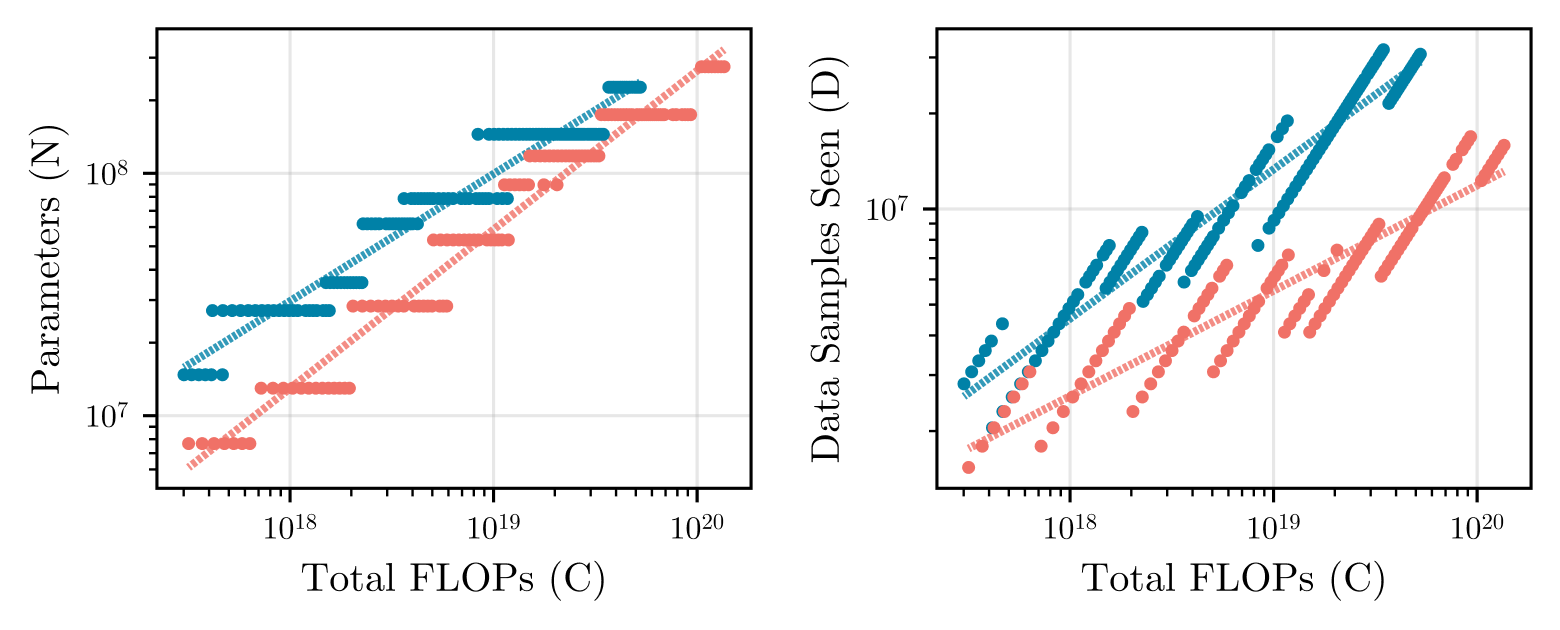
\includegraphics[width=\linewidth]{images/data_param_laws_fix.png}
    \vspace{-0.5cm}
    \caption{
        \textbf{Data and Model Scaling Plots.} 
        While our model~(\textcolor[HTML]{0081A7}{blue}) is optimal when sufficient data is available, decoder-only LVSM~(\textcolor[HTML]{F07167}{red}) performs better with less data. The Pareto frontier analysis shows that our model is more data-hungry. Our model is also less parameter-efficient, although the gap closes as we increase the training compute. However, with sufficient data and compute, our model~(\textcolor[HTML]{0081A7}{blue}) is overall superior in terms of training compute-optimality and rendering speed.
        \vspace{-1\baselineskip}
    }
    \label{fig:opt-model-scaling}
\end{figure}
